\RequirePackage{luatex85}
\documentclass[border=1pt]{standalone}

\usepackage{tikz}
\usetikzlibrary{arrows, patterns}

\def\hexagonsize{0.4cm}
\pgfdeclarepatternformonly
	{hexagons}% name
	{\pgfpointorigin}% lower left
	{\pgfpoint{3*\hexagonsize}{0.866025*2*\hexagonsize}}%  upper right
	{\pgfpoint{3*\hexagonsize}{0.866025*2*\hexagonsize}}%  tile size
	{% shape description
	  \pgfsetlinewidth{0.4pt}
	  \pgftransformshift{\pgfpoint{0mm}{0.866025*\hexagonsize}}
	  \pgfpathmoveto{\pgfpoint{0mm}{0mm}}
	  \pgfpathlineto{\pgfpoint{0.5*\hexagonsize}{0mm}}
	  \pgfpathlineto{\pgfpoint{\hexagonsize}{-0.866025*\hexagonsize}}
	  \pgfpathlineto{\pgfpoint{2*\hexagonsize}{-0.866025*\hexagonsize}}
	  \pgfpathlineto{\pgfpoint{2.5*\hexagonsize}{0mm}}
	  \pgfpathlineto{\pgfpoint{3*\hexagonsize+0.2mm}{0mm}}
	  \pgfpathmoveto{\pgfpoint{0.5*\hexagonsize}{0mm}}
	  \pgfpathlineto{\pgfpoint{\hexagonsize}{0.866025*\hexagonsize}}
	  \pgfpathlineto{\pgfpoint{2*\hexagonsize}{0.866025*\hexagonsize}}
	  \pgfpathlineto{\pgfpoint{2.5*\hexagonsize}{0mm}}
	  \pgfusepath{stroke}
	}

\tikzstyle{myarrow} = [<<->>, shorten >=4pt, shorten <=4pt, thick, line width=4pt]


\begin{document}
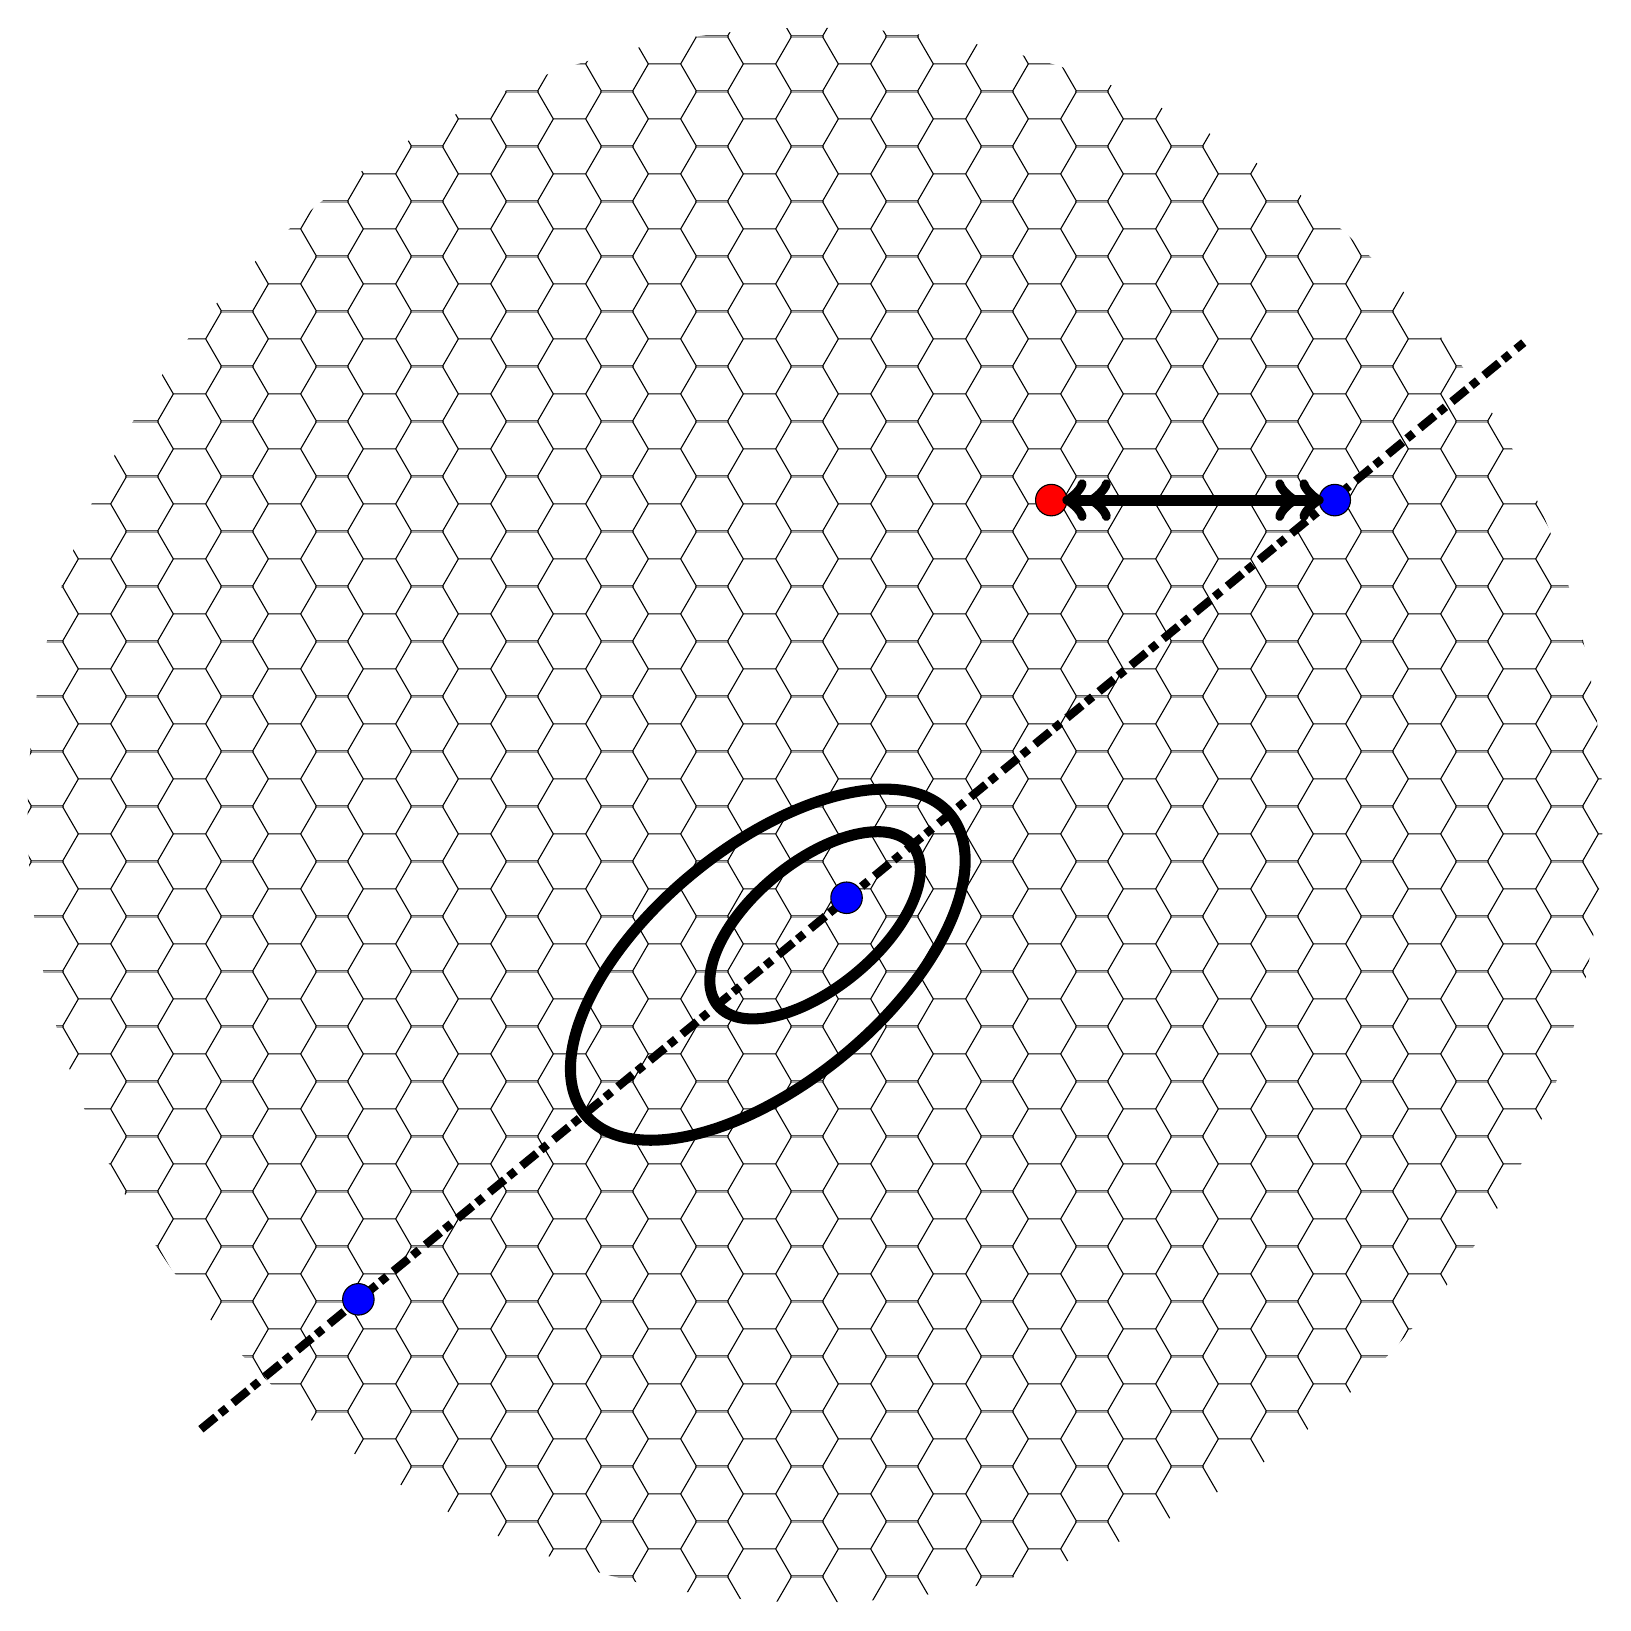
\begin{tikzpicture}
  %camera achse
  \draw[line width=3pt,,dash pattern={on 7pt off 2pt on 3pt off 3pt}] (-7.8,-7.8) -- (9,6);
  %zeichnet hexagonales Rundes Grid
  \fill[pattern=hexagons] (0,0) circle (10cm);
  %position expected source
  \filldraw[fill=blue] (6.6, 4) circle [radius=0.2];
  %position measured source 
  \filldraw[fill=red] (3,4) circle [radius=0.2];
  %theta2
  \draw[myarrow] (3,4) -- (6.6,4);

  \draw[line width=4pt] (-0.6,-1.9) circle [x radius=30mm, y radius=15mm, rotate=39.4];
  \draw[line width=4pt] (0,-1.4) circle [x radius=16mm, y radius=8mm, rotate=39.4];
  \filldraw[fill=blue] (0.4, -1.05) circle [radius=0.2];
  
  \filldraw[fill=blue] (-5.8, -6.15) circle [radius=0.2];


\end{tikzpicture}
\end{document}
